\boxde
\Opensolutionfile{ans}[ans/2D1-5-DEON-1]
\begin{ex}%[2D1Y5-1]
    Bảng biến thiên sau đây là của hàm số nào?
    \begin{center}
        
\begin{tikzpicture}[>=stealth]
            \tkzTabInit[nocadre=false,lgt=1,espcl=2,deltacl=0.5]{$x$/.7 ,$y'$/.7,$y$/2}
            {$-\infty$ , $1$ , $+\infty$}
            \tkzTabLine{ , + , $0$ , + , }
            \tkzTabVar{-/$-\infty$ , R , +/$+\infty$}
            \tkzTabIma{1}{3}{2}{$1$}
        \end{tikzpicture}
    \end{center}
    \choice
    {$y=-x^3+3x^2-3x$}
    {$y=-x^3-3x^2-3x$}
    {$y=x^3+3x^2-3x$}
    {\True $y=x^3-3x^2+3x$}
    \loigiai{
        $y=x^3-3x^2+3x\Rightarrow y'=3x^2-6x+3\Rightarrow y'=0\Leftrightarrow x=1$.}
\end{ex}
\begin{ex}%[2D1Y5-1]
    \immini
    {
        Đường cong hình bên là đồ thị của hàm số nào trong bốn hàm số ở phương án A, B, C, D dưới đây?
        \choice
        { $ y=x^3-3x-1$}
        {$ y=-x^3+3x^2+1$}
        {$ y=-x^3-3x^2-1$}
        {\True $ y=x^3-3x+1$}
    }
    {
        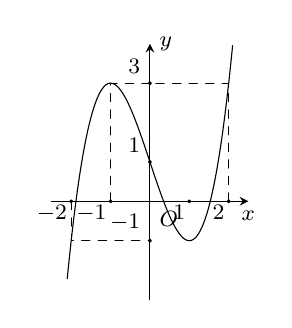
\begin{tikzpicture}[line join = round, line cap = round,>=stealth,x = 1cm,y = 1cm,font=\footnotesize,scale=.5]
            %Vẽ hệ trục Oxy
            \draw[->] (-2.5,0)--(0,0) node[below right]{$O$}--(2.5,0) node[below]{$x$};
            \draw[->] (0,-2.5)--(0,4) node[right]{$y$};
            %Vẽ các điểm trên hệ trục
            \foreach \x in {-2,-1,1,2} \draw[fill=black] (\x,0) node [below left=-2pt] {$\x$} circle (1pt);
            \foreach \y in {-1,1,3} \draw[fill=black] (0,\y) node [above left] {$\y$} circle (1pt);
            %Vẽ đồ thị hàm số
            \draw[samples=200,domain=-2.1:2.1,smooth] plot (\x, {(\x)^3-3*(\x)+1});
            \draw[dashed](-2,0)--(-2,-1)--(0,-1) (-1,0)--(-1,3)--(0,3) (2,0)--(2,3)--(0,3);
        \end{tikzpicture}
    }
    \loigiai{
        Từ đồ thị ta thấy hệ số $a > 0$ do nhánh phải hướng lên trên.\\
        Mặt khác đồ thị cắt trục tung tại $A(0;1)$ nên hàm số thỏa mãn là $y=x^3-3x+1$.
    }
\end{ex}
\begin{ex}%[2D1Y5-1]
    Đường cong trong hình bên dưới là đồ thị của hàm số nào dưới đây?
    \begin{center}
        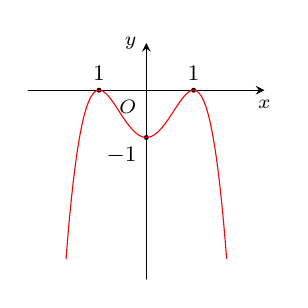
\begin{tikzpicture}[>=stealth, line join=round, line cap=round, font=\footnotesize, scale=.6]
            \def\a{-1} % Hệ số a phải khác 0
            \def\b{2}
            \def\c{-1}
            \draw[->] (-2.5,0) -- (2.5,0) node[below] {\scriptsize $x$};
            \draw[->] (0,-4) -- (0,1) node[left] {\scriptsize $y$};
            \draw (0,0)node[below left]{\scriptsize $O$};
            \foreach \x in {-1,1}\fill (\x,0)circle(1.5pt)node[above]{$1$};
            \fill (0,-1)circle(1.5pt)node[below left]{$-1$};
            \draw[red,samples=150,smooth,domain=-1.7:1.7] plot(\x,{\a*(\x)^4+(\b)*(\x)^2+(\c)});
        \end{tikzpicture}
    \end{center}
    \choice
    {$y=-x^4+3x^2-3$}
    {$y=-x^4+3x^2-2$}
    {\True $y=-x^4+2x^2-1$}
    {$y=-x^4+x^2-1$}
    \loigiai{
        Ta thấy đồ thị của hàm số cắt trục tung tại điểm có tọa độ $(0;-1)$ nên hệ số tự do là $-1$.\\
        Vì đồ thị của hàm số đi qua điểm $(1;0)$ nên hàm số có đồ thị như hình trên là $y=-x^4+2x^2-1$.
    }
\end{ex}
\begin{ex}%[2D1Y5-1]
    Hàm số $y=-x^3+3x^2-1$ có đồ thị nào trong các đồ thị dưới đây?
    \begin{center}
        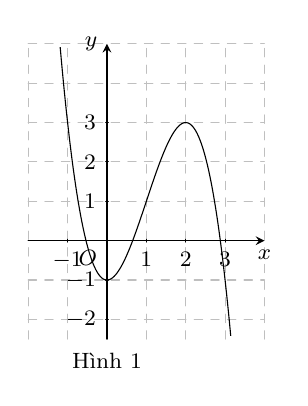
\begin{tikzpicture}[scale=.5,>=stealth, font=\footnotesize, line join=round, line cap=round]
            \def\a{-1} \def\b{3} \def\c{0} \def\d{-1} % Hệ số
            \def\xmin{-2} \def\xmax{4}
            \def\ymin{-2.5} \def\ymax{5}
            \draw[color=gray!50,dashed] (\xmin,\ymin) grid (\xmax,\ymax);
            \draw[->] (\xmin,0)--(\xmax,0) node [below]{$x$};
            \draw[->] (0,\ymin)--(0,\ymax) node [left]{$y$};
            \node at (0,0) [below left]{$O$};
            \node at (0,-2.6) [below]{Hình $1$};
            \clip (\xmin+0.1,\ymin+0.1) rectangle (\xmax-0.5,\ymax-0.1);
            \draw[smooth,samples=300] plot(\x,{\a*(\x)^3+\b*(\x)^2+\c*(\x)+\d});
            \foreach \x in {-1,1,2,3}
            \draw[thin] (\x,1pt)--(\x,-1pt) node [below] {$\x$};
            \foreach \y in {-2,-1,1,2,3}
            \draw[thin] (1pt,\y)--(-1pt,\y) node [left] {$\y$};
        \end{tikzpicture}
        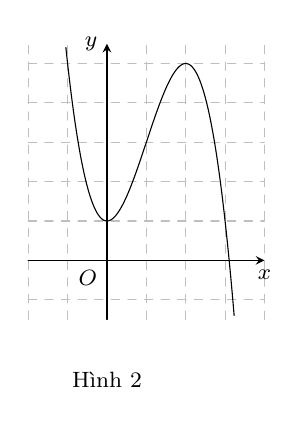
\begin{tikzpicture}[scale=.5,>=stealth, font=\footnotesize, line join=round, line cap=round]
            \def\a{-1} \def\b{3} \def\c{0} \def\d{1} % Hệ số
            \def\xmin{-2} \def\xmax{4}
            \def\ymin{-1.5} \def\ymax{5.5}
            \draw[color=gray!50,dashed] (\xmin,\ymin) grid (\xmax,\ymax);
            \draw[->] (\xmin,0)--(\xmax,0) node [below]{$x$};
            \draw[->] (0,\ymin)--(0,\ymax) node [left]{$y$};
            \node at (0,0) [below left]{$O$};
            \node at (0,-2.6) [below]{Hình $2$};
            \clip (\xmin+0.1,\ymin+0.1) rectangle (\xmax-0.5,\ymax-0.1);
            \draw[smooth,samples=300] plot(\x,{\a*(\x)^3+\b*(\x)^2+\c*(\x)+\d});
        \end{tikzpicture}
        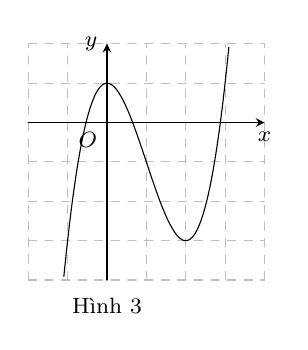
\begin{tikzpicture}[scale=.5,>=stealth, font=\footnotesize, line join=round, line cap=round]
            \def\a{1} \def\b{-3} \def\c{0} \def\d{1} % Hệ số
            \def\xmin{-2} \def\xmax{4}
            \def\ymin{-4} \def\ymax{2}
            \draw[color=gray!50,dashed] (\xmin,\ymin) grid (\xmax,\ymax);
            \draw[->] (\xmin,0)--(\xmax,0) node [below]{$x$};
            \draw[->] (0,\ymin)--(0,\ymax) node [left]{$y$};
            \node at (0,0) [below left]{$O$};
            \node at (0,-4.2) [below]{Hình $3$};
            \clip (\xmin+0.1,\ymin+0.1) rectangle (\xmax-0.5,\ymax-0.1);
            \draw[smooth,samples=300] plot(\x,{\a*(\x)^3+\b*(\x)^2+\c*(\x)+\d});
        \end{tikzpicture}
        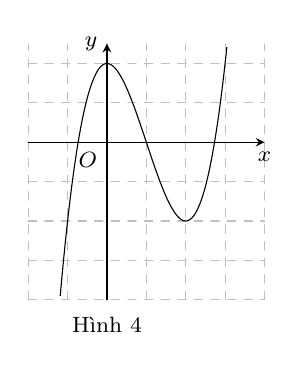
\begin{tikzpicture}[scale=.5,>=stealth, font=\footnotesize, line join=round, line cap=round]
            \def\a{1} \def\b{-3} \def\c{0} \def\d{2} % Hệ số
            \def\xmin{-2} \def\xmax{4}
            \def\ymin{-4} \def\ymax{2.5}
            \draw[color=gray!50,dashed] (\xmin,\ymin) grid (\xmax,\ymax);
            \draw[->] (\xmin,0)--(\xmax,0) node [below]{$x$};
            \draw[->] (0,\ymin)--(0,\ymax) node [left]{$y$};
            \node at (0,0) [below left]{$O$};
            \node at (0,-4.2) [below]{Hình $4$};
            \clip (\xmin+0.1,\ymin+0.1) rectangle (\xmax-0.5,\ymax-0.1);
            \draw[smooth,samples=300] plot(\x,{\a*(\x)^3+\b*(\x)^2+\c*(\x)+\d});
        \end{tikzpicture}
    \end{center}
    \choice
    {\True Hình $1$}
    {Hình $4$}
    {Hình $2$}
    {Hình $3$}
    \loigiai{Do đồ thị có giao điểm với trục tung là $\left(0;-1\right)$ nên ta chọn Hình $1$.
    }
\end{ex}
\begin{ex}%[2D1Y5-1]
    \immini{
        Đường cong ở hình bên là đồ thị của một trong bốn hàm số dưới đây. Hàm số đó là hàm số nào?
        \choice
        {$y=x^{4}-2x^2+1$}
        {\True $y=x^3-3x+1$}
        {$y=-x^3+3x+1$}
        {$y=x^3-3x^2+1$}}{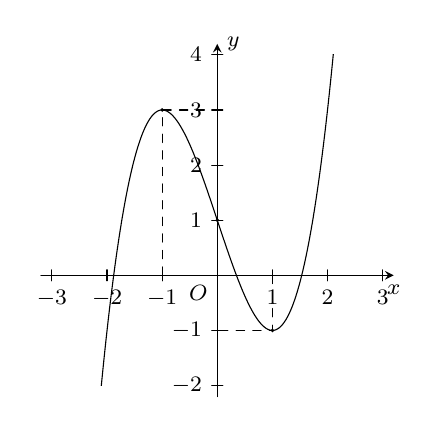
\begin{tikzpicture}[scale=0.7, font=\footnotesize, line join=round, line cap=round, >=stealth]
            \def\xmin{-3}\def\xmax{3}\def\ymin{-2}\def\ymax{4}
            \draw[->] (\xmin-0.2,0)--(\xmax+0.2,0) node[below] {\footnotesize $x$};
            \draw[->] (0,\ymin-0.2)--(0,\ymax+0.2) node[right] {\footnotesize $y$};
            \draw (0,0) node [below left] {\footnotesize $O$};
            \foreach \x in {-3,-2,-1,1,2,3}\draw (\x,0.1)--(\x,-0.1) node [below] {\footnotesize $\x$};
            \foreach \y in {-2,-1,1,2,3,4}\draw (0.1,\y)--(-0.1,\y) node [left] {\footnotesize $\y$};
            \clip (\xmin,\ymin) rectangle (\xmax,\ymax);
            \draw[smooth,samples=200,domain=\xmin:\xmax] plot (\x,{1*((\x)^3)+0*((\x)^2)+-3*(\x)+1});
            \draw[dashed] (0.0,0)--(0.0,1.0)--(0,1.0);\fill (0.0,1.0) circle (1pt);
            \draw[dashed] (-1.0,0)--(-1.0,3.0)--(0,3.0);\fill (-1.0,3.0) circle (1pt);
            \draw[dashed] (1.0,0)--(1.0,-1.0)--(0,-1.0);\fill (1.0,-1.0) circle (1pt);
    \end{tikzpicture}}
    \loigiai{Đây là đồ thị của hàm số bậc ba, có $a>0$ và đi qua điểm $(-1;3)$.\\
        Cho nên chỉ có đáp án $y= x^3 -3x+1$ thoả mãn.}
\end{ex}
\begin{ex}%[2D1B5-1]
    Đồ thị của hàm số nào dưới đây có dạng như đường cong trong hình bên dưới?
    \begin{center}
        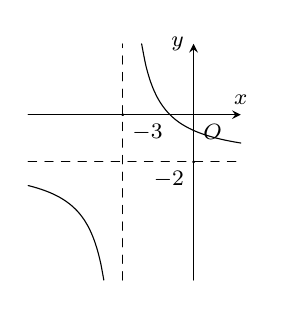
\begin{tikzpicture}[scale=.3, font=\footnotesize, line join=round, line cap=round, >=stealth]
            \draw[->] (-7,0)--(0,0) node[below
            right]{$O$}--(2,0)
            node[above]{$x$};
            \draw[->] (0,-7)--(0,3)
            node[left]{$y$};
            \draw[smooth]
            plot[domain=-2.2:2]
            (\x,{(2*(\x)+2)/(-(\x)-3)});
            \draw[smooth]
            plot[domain=-7:-3.8]
            (\x,{(2*(\x)+2)/(-(\x)-3)});
            \draw[dashed] (-3,-7)--(-3,3);
            \draw[dashed] (-7,-2)--(2,-2);
            \path
            (0,-2)node[below left]{$-2$}
            (-3,0)node[below right]{$-3$}
            ;
            \draw[fill](0,-2)circle(1pt);
            \draw[fill](-3,0)circle(1pt);
        \end{tikzpicture}
    \end{center}
    \choice
    {\True $y=\dfrac{2x+2}{-x-3}$}
    {$y=\dfrac{x+2}{x-3}$}
    {$y=x^3-\dfrac{2}{3}$}
    {$y=x^4-2x-\dfrac{2}{3}$}
    \loigiai{
        \begin{itemize}
            \item Tiệm cận đứng $x=-3$.
            \item Tiệm cận ngang $y=-2$.
        \end{itemize}
        Do đó, hàm số cần tìm là $y=\dfrac{2x+2}{-x-3}$.
    }
\end{ex}
\begin{ex}%[2D1B5-1]
    \immini{Cho hàm số $ y=ax^3+bx^2+cx+d$ có đồ thị như hình bên. Trong các giá trị $ a$, $b$, $c$, $d$ có bao nhiêu giá trị âm.
        \choice
        {\True $ 2 $}
        {$ 1 $}
        {$ 4 $}
        {$ 3 $}}{
        \begin{tikzpicture}[>=stealth,line join=round,line cap=round,font=\scriptsize,scale=0.65]
            \draw [->] (-3,0)--(4,0)node[below]{$ x $};
            \draw [->] (0,-2)--(0,3)node[left]{$ y $};
            \draw [smooth,domain=-2:3.4] plot(\x,{-(\x)^3/3+3*(\x)^2/4+(\x)-1});
            \draw [fill=black] (0,0)node[below left]{$ O $}circle(1pt);
        \end{tikzpicture}
    }
    \loigiai{
        Đồ thị có hướng đi xuống nên $ a<0$.\\
        Giao của đồ thị với trục tung tại điểm có tung độ âm nên $ d<0$.\\
        Gọi $ x_1$, $ x_2 $ lần lượt là hai điểm cực trị của hàm số.\\
        Do $ x_1\cdot x_2<0$ nên $ a\cdot c<0$ nên $ c>0$.\\
        Hơn nữa $ x_1+x_2>0$ nên $\dfrac{-b}{3a}>0\Rightarrow b>0.$\\
        Vậy có hai hệ số âm.
    }
\end{ex}
\begin{ex}%[2D1B5-1]
    \immini{
        Đồ thị hàm số nào dưới đây có dạng như đường cong trong hình vẽ bên?
        \choice
        {$y=x^4-2x^2+1$}
        {\True $y=-x^4+2x^2+1$}
        {$y=x^4+3x^2+1$}
        {$y=-x^4+3x^2+1$}
    }{
        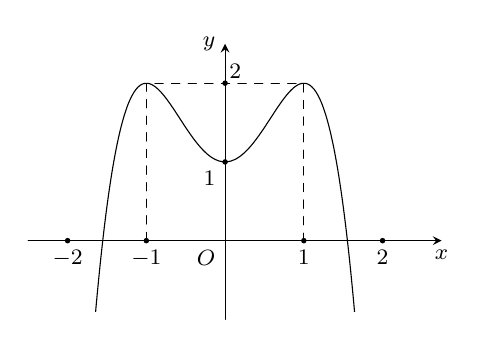
\begin{tikzpicture}[scale=1,>=stealth, font=\footnotesize, line join=round, line cap=round]
            \def\xmin{-2.5} \def\xmax{2.75}
            \def\ymin{-1} \def\ymax{2.5}
            \draw[->] (\xmin,0)--(\xmax,0) node [below]{$x$};
            \draw[->] (0,\ymin)--(0,\ymax) node [left]{$y$};
            \node at (0,0) [below left]{$O$};
            \clip (\xmin+0.1,\ymin+0.1) rectangle (\xmax-0.5,\ymax-0.1);
            \draw[smooth,samples=200] plot(\x,{-(\x)^4+2*(\x)^2+1});
            \foreach \x in {-2,-1,1,2}{
                \fill (\x,0) node[below]{$\x$} circle (1pt);
            }
            \fill (0,1) node[below left]{$1$} circle (1pt);
            \fill (0,2) node[above right=-2pt]{$2$} circle (1pt);
            \draw[dashed] (-1,0)|-(0,2)-|(1,0);
        \end{tikzpicture}
    }
    \loigiai{
        Dựa vào đồ thị, hàm số đã cho là hàm trùng phương có hệ số $a<0$ và đi qua điểm $\left(1;2\right)$.\\
        Xét hàm số $y=-x^4+2x^2+1$ có $y\left(1\right)=-1+2+1=2$ nên đồ thị đi qua điểm $\left(1;2\right)$. Vậy hàm số có đồ thị như hình vẽ là $y=-x^4+2x^2+1$.
    }
\end{ex}
\begin{ex}%[2D1B5-1]
    Cho các đường cong $(C_1)\colon y=x^3-3x^2+4$, $(C_2)\colon y=-x^4+x^2-3$ và $(C_3)\colon y=\dfrac{5x+2}{x-1}$. Hỏi các đường cong nào có tâm đối xứng?
    \choice
    {$(C_1)$, $(C_2)$ và $(C_3)$}
    {\True $(C_1)$ và $(C_3)$}
    {$(C_2)$ và $(C_3)$}
    {$(C_1)$ và $(C_2)$}
    \loigiai{
        $(C_1)$ có hoành độ tâm đối xứng là nghiệm của $y''=0$ và $(C_3)$ có tâm đối xứng là giao hai tiệm cận. }
\end{ex}
\begin{ex}%[2D1B5-1]
    \immini{Cho hàm số $y=a x^3+bx^2+cx+d$ $(a\not=0)$ có đồ thị như hình vẽ bên. Chọn khẳng định đúng?
        \choice
        { $a>0, d>0$}
        { $a>0, b<0, c>0$}
        { $a>0, b>0, c>0, d>0$}
        {\True $a>0, c<0, d>0$}
    }{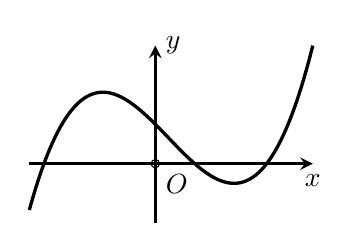
\begin{tikzpicture}[>=stealth,x=2cm,y=1cm,scale=.5]
            \draw[->,line width = 1pt] (-1.6,0)--(0,0)%
            node[below right]{$O$}--(2,0) node[below]{$x$};
            \draw[->,line width = 1pt] (0,-1.5) --(0,3) node[right]{$y$};
            %\foreach \x in {-2,-1,1,2}{	\draw (\x,0) node[below,blue]{$\x$} circle (1pt);%Ox}
            %\foreach \y in {-1,1,2,3}{	\draw (0,\y) node[left,blue]{$\y$} circle (1pt);%Oy }
            \draw [ line width = 1.2pt, domain=-1.6:2, samples=100]%
            plot (\x, {(\x)^3-0.5*(\x)^2-2 *(\x)+1});
            \draw[fill=none] (0,0) circle(3pt);
    \end{tikzpicture}}
    \loigiai{
        + Hàm số đi từ dưới lên nên $a>0$.\\
        + Đồ thị cắt trục $Oy$ tại điểm có tung độ dương nên $d>0$.\\
        + Hàm số có hai cực trị trái dấu nên $a\cdot c<0$ hay $c<0.$\\
        Vậy đồ thị hàm số đã cho có tính chất $a>0, c<0, d>0$.
    }
\end{ex}
\begin{ex}%[2D1K5-1]
    \immini
    {
        Cho hàm số $y=ax^3+bx^2+cx+d$ có đồ thị như hình bên. Trong các số $a$, $b$, $c$, $d$ có bao nhiêu số dương?
        \choice
        {$1$}
        {$0$}
        {\True $2$}
        {$3$}
    }
    {
        \begin{tikzpicture}[scale=.8, font=\footnotesize, line join=round, line cap=round, >=stealth]
            \def\a{-1}
            \def\b{1}
            \def\c{1.75}
            \def\d{-1}
            \draw[->] (-2,0) -- (3,0)node[below]{\footnotesize $x$};
            \draw[->] (0,-2) -- (0,2) node[left] {\footnotesize $y$};
            \draw[fill=black] (0,0)node[below left]{\footnotesize $O$} circle(1pt);
            \clip (-2,-2)rectangle(3,2);
            \draw[samples=150,smooth,domain=-2:3] plot(\x,{\a*(\x)^3+(\b)*(\x)^2+(\c)*\x+(\d)});
        \end{tikzpicture}
    }
    \loigiai{
        Ta có $y'=3ax^2+2bx+c$.\\
        Từ đồ thị suy ra
        \begin{itemize}
            \item $\lim \limits_{x \to +\infty} f(x)=-\infty\Rightarrow a<0$.
            \item đồ thị cắt trục $Oy$ tại điểm có tung độ âm nên $d<0$.
            \item hàm số có hai cực trị trái dấu và tổng hai hoành độ cực trị dương nên
            $$\heva{& -\dfrac{2b}{3a}>0 \\ & \dfrac{c}{3a}<0}\Leftrightarrow \heva{& b>0 \\ & c>0} (\text{vì } a<0).$$
        \end{itemize}
        Vậy trong các số $a$, $b$, $c$, $d$ có $2$ số dương.
    }
\end{ex}
\begin{ex}%[2D1K5-1]
    \immini
    {
        Cho hàm số bậc ba $y=f(x)$, đồ thị của hàm số $y=f'(x)$ có dạng như hình vẽ bên. Hỏi đồ thị hàm số $y=f(x)$ là đồ thị nào trong các hình sau?
    }
    {
        \begin{tikzpicture}[scale=0.6,font=\footnotesize, line join=round, line cap=round, >=stealth]
            \draw[->] (-1,0)--(4,0) node[below right]{$x$};
            \draw[->] (0,-3.5)--(0,1) node[above right]{$y$};
            \draw[samples=100] plot[domain=-.3:3.3] (\x, {-(\x-1)*(\x-2)});
            \draw[fill=black] (1,0) circle(1pt) node[above left]{$1$};
            \draw[fill=black] (2,0) circle(1pt) node[above right]{$2$};
            \draw[fill=black] (0,0) circle(1pt) node[below left]{$O$};
        \end{tikzpicture}
    }
    \begin{center}
        \begin{tikzpicture}[scale=0.7,font=\footnotesize, line join=round, line cap=round, >=stealth]
            \draw[->] (-.5,0)--(4,0) node[below right]{$x$};
            \draw[->] (0,-1)--(0,4) node[above right]{$y$};
            \draw[samples=100] plot[domain=-.3:3.3] (\x, {(\x)^3/3 - 3*(\x)^2/2+2*\x});
            \draw[fill=black] (1,0) circle(1pt) node[below]{$1$};
            \draw[fill=black] (2,0) circle(1pt) node[below]{$2$};
            \draw[fill=black] (3,0) circle(1pt) node[below]{$3$};
            \draw[fill=black] (0,0) circle(1pt) node[above left]{$O$};
            \draw (2,-2) node{\text{Hình 1}};
            \begin{scope}[shift={(6,0)}]
                \draw[->] (-.5,0)--(4,0) node[below right]{$x$};
                \draw[->] (0,-1)--(0,4) node[above right]{$y$};
                \draw[samples=100] plot[domain=-.3:3.3] (\x, {-(\x)^3/3 + 3*(\x)^2/2-2*\x+2});
                \draw[fill=black] (1,0) circle(1pt) node[below]{$1$};
                \draw[fill=black] (2,0) circle(1pt) node[below]{$2$};
                \draw[fill=black] (3,0) circle(1pt) node[below]{$3$};
                \draw[fill=black] (0,0) circle(1pt) node[above left]{$O$};
                \draw (2,-2) node{\text{Hình 2}};
            \end{scope}
            \begin{scope}[shift={(12,0)}]
                \draw[->] (-.5,1.5)--(4,1.5) node[below right]{$x$};
                \draw[->] (0,-1)--(0,4) node[above right]{$y$};
                \draw[samples=100] plot[domain=-.3:3.7] (\x, {-(\x)^3/3 + 2*(\x)^2-3*\x+1});
                \draw[fill=black] (1,1.5) circle(1pt) node[above]{$1$};
                \draw[fill=black] (2,1.5) circle(1pt) node[above]{$2$};
                \draw[fill=black] (3,1.5) circle(1pt) node[above]{$3$};
                \draw[fill=black] (0,1.5) circle(1pt) node[below left]{$O$};
                \draw (2,-2) node{\text{Hình 3}};
            \end{scope}
            \begin{scope}[shift={(18,0)}]
                \draw[->] (-.5,1.5)--(4,1.5) node[below right]{$x$};
                \draw[->] (0,-1)--(0,4) node[above right]{$y$};
                \draw[-] (-1,2.5)--(1,0)--(2,1.5)--(3.25,-1);
                \draw[fill=black] (1,1.5) circle(1pt) node[above]{$1$};
                \draw[fill=black] (2,1.5) circle(1pt) node[above]{$2$};
                \draw[fill=black] (3,1.5) circle(1pt) node[above]{$3$};
                \draw[fill=black] (0,1.5) circle(1pt) node[below left]{$O$};
                \draw (2,-2) node{\text{Hình 4}};
            \end{scope}
        \end{tikzpicture}
    \end{center}
    \choice
    {Hình $1$}
    {\True Hình $2$}
    {Hình $3$}
    {Hình $4$}
    \loigiai{
        Do $y=f(x)$ là hàm bậc ba nên $y=f'(x)$ là hàm bậc hai.\\
        Dựa vào đồ thị thì hàm bậc hai $y=f'(x)$ nhận $1$, $2$ là nghiệm và đồ thị là parabol hướng xuống nên $y=f'(x)=a(x-1)(x-2)=ax^2-3ax+2a$ với $a<0$.\\
        Từ đó ta có $f(x) = \displaystyle\int f'(x) \mathrm{\,d}x = \dfrac{a}{3}x^3 - \dfrac{3a}{2}x^2 + 2ax + C$.\\
        Hàm số $f(x)$ có hai điểm cực trị là $x=1$, $x=2$ và $\lim\limits_{x\to +\infty} f(x) = -\infty$ nên chọn đáp án là hình $2$.
    }
\end{ex}
\begin{ex}%[2D1K5-1]
    Cho hàm số $y=ax^3+bx^2+cx+d$ đạt cực trị tại các điểm $x_1,x_2$ thỏa mãn $x_1\in(-1;0)$, $x_2\in(1;2)$ biết rằng hàm số đồng biến trên khoảng $(x_1;x_2)$. Đồ thị hàm số cắt trục tung tại điểm có tung độ âm. Trong các khẳng định sau, khẳng định nào đúng?
    \choice
    {\True $a<0, b>0, c>0, d<0$}
    {$a<0, b<0, c>0, d<0$}
    {$a>0, b>0, c>0, d<0$}
    {$a<0, b>0, c<0, d<0$}
    \loigiai{
        Vì hàm số $y=ax^3+bx^2+cx+d$ đạt cực trị tại các điểm $x_1, x_2$ và đồng biến trên khoảng $(x_1;x_2)$ nên $a<0$.\\
        Đồ thị hàm số cắt trục tung tai điểm có tung độ âm nên $d<0$.\\
        Hàm số có hai điểm cực trị thỏa $x_1\in(-1;0), x_2\in(1;2)$ nên $y'=3ax^2+2bx+c=0$ có hai nghiệm trái dấu nên $a.c<0\Rightarrow c>0$.\\
        Mặt khác $y'=0$ có tổng hai nghiệm dương nên $-\dfrac{b}{a}>0\Rightarrow b>0$.}
\end{ex}
\begin{ex}%[2D1K5-1]
    \immini{Cho hàm số $y=(a-1)x^4+(b+2)x^2+c-1$ có đồ thị như hình vẽ bên. Mệnh đề nào dưới đây đúng?
        \choice
        {$a>1,b>-2,c>1$}
        {\True $a>1,b<-2,c>1$}
        {$a<1,b>-2,c>1$}
        {$a>1,b<2,c>1$}
    }{
        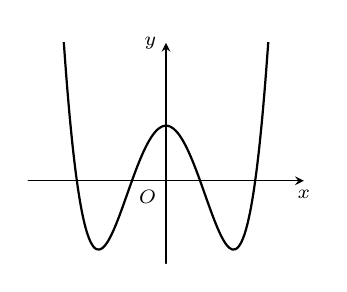
\begin{tikzpicture}[>=stealth,line join=round, line cap=round, font=\footnotesize,scale=.7]
            \def\a{1} % Hệ số a phải khác 0
            \def\b{-3}
            \def\c{1}
            \draw[->] (-2.5,0) -- (2.5,0) node[below] {\scriptsize $x$};
            \draw[->] (0,-1.5) -- (0,2.5) node[left] {\scriptsize $y$};
            \draw (0,0)node[below left]{\scriptsize $O$};
            \clip (-2.5,-1.5)rectangle(2.5,2.5);
            \draw[thick,samples=150,smooth,domain=-4:4] plot(\x,{\a*(\x)^4+(\b)*(\x)^2+(\c)});
        \end{tikzpicture}
    }
    \loigiai{
        Dựa theo hình vẽ, đồ thị hàm số đã cho có $a-1>0\Leftrightarrow a>1$.\\
        Đồ thị hàm số đi qua điểm trên trục tung có tung độ dương nên $c-1>0\Leftrightarrow c>1$.\\
        Đồ thị hàm số có $3$ cực trị nên $(a-1)\cdot (b+2)<0$. Suy ra $b+2<0\Leftrightarrow b<-2$.
    }
\end{ex}
\begin{ex}%[2D1K5-1]
    \immini{Cho hàm số $ f(x)=ax^4+bx^2+c $ ($ a\ne 0 $) có đồ thị như hình vẽ.
        Tìm mệnh đề đúng trong các mệnh đề sau.
        \choice
        { $ a>0, b<0, c>0 $ }
        { $ a<0, b>0, c<0 $ }
        { $ a<0, b<0, c>0 $ }
        {\True $ a<0, b>0, c>0 $ }}
    {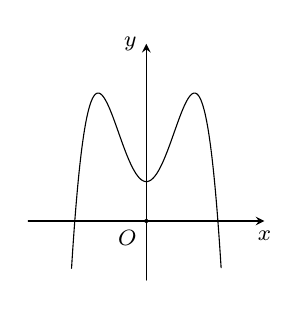
\begin{tikzpicture}[>=stealth,line join=round,line cap=round,font=\footnotesize,scale=0.5]
            \draw[->] (0,-1.5)--(0,4.5)node[left]{$y$};
            \foreach \y in {}
            \draw[shift={(0,\y)}] (2pt,0)--(-2pt,0) node[left] {\footnotesize $\y$};
            \draw[->] (-3,0)--(3,0)node[below]{$x$};
            \foreach \x in {}
            \draw[shift={(\x,0)}] (0,2pt)--(0,-2pt) node[below] {\footnotesize $\x$};
            \fill (0,0) node[below left]{\footnotesize $O$} circle(1.5pt);
            \draw[samples=150,smooth,domain=-1.9:1.9] plot(\x,{-(\x)^4+3*(\x)^2+1});
    \end{tikzpicture}}
    \loigiai{
        Từ đồ thị hàm số, ta có $ \lim\limits_{x \to \pm \infty} f(x) =\lim \limits_{x \to \pm \infty} (ax^4)=-\infty$. Suy ra $ a<0 $.\\
        Đồ thị hàm số cắt trục tung tại điểm $ (0;c) $, suy ra $ c>0 $.\\
        Đồ thị hàm số có ba điểm cực trị nên $ ab <0 $, suy ra $ b>0 $.
    }
\end{ex}
\begin{ex}%[2D1B5-3]
    \immini{
        Cho hàm số $y = f(x)$ có đồ thị là đường cong trong hình vẽ bên. Số nghiệm của phương tình $f(x) -m + 6 = 0$ với $m > 3$ là
        \choice
        {$4$}
        {\True $2$}
        {$3$}
        {$1$}
    }{
        \begin{tikzpicture}[scale=0.7, font=\footnotesize, line join=round, line cap=round, >=stealth,yscale=0.7]
            \def \xmin{-3}
            \def \xmax{3}
            \def \ymin{-5}
            \def \ymax{1.5}
            \draw[->] (\xmin,0)--(\xmax,0) node[below] {$x$};
            \draw[->] (0,\ymin)--(0,\ymax) node[left] {$y$};
            \draw[fill] (0,0) node [below right] {$O$} circle(1.3 pt);
            \draw[fill] (0,-3) node [above left] {$-3$} circle(1.3 pt);
            \draw[fill] (0,-4) node [left] {$-4$} circle(1.3 pt);
            \begin{scope}
                \clip (\xmin+0.01,\ymin+0.01) rectangle (\xmax-0.01,\ymax-0.01);
                \draw[samples=350,domain=\xmin+0.01:\xmax-0.01,smooth,variable=\x] plot (\x,{(\x)^4-2*(\x)^2-3});
            \end{scope}
            % \begin{scope}[on background layer]\path[white]node{MDD-108};\end{scope}
        \end{tikzpicture}
    }
    \loigiai{
        Ta có $f(x) -m + 6 = 0 \Leftrightarrow f(x) = m-6. \qquad (1)$\\
        Số nghiệm của phương trình $(1)$ là số giao điểm của đồ thị hàm số $y=f(x)$ và đường thẳng $y = m-6$.\\
        Vì $m > 3$ nên $m - 6 > -3$.\\
        Dựa vào đồ thị ta thấy, phương trình đã cho có $2$ nghiệm.
    }
\end{ex}
\begin{ex}%[2D1B5-3]
    \immini{Cho hàm số $y=f(x)$ có bảng biến thiên như hình bên. Số nghiệm của phương trình $f(x)=f(0)$ là
        \choice
        {$2$}
        {\True $3$}
        {$1$}
        {$0$}}
    {
        
\begin{tikzpicture}[>=stealth]
            \tkzTabInit[nocadre=false,lgt=1,espcl=2,deltacl=0.5]
            {$x$/.6 ,$y'$/.6,$y$/2}
            {$-\infty$ , $-1$ , $3$ , $+\infty$}
            \tkzTabLine{ , + , $0$ , - , $0$ , + , }
            \tkzTabVar{-/$-\infty$ , +/$2$ , -/$1$ , +/$+\infty$}
        \end{tikzpicture}
    }
    \loigiai{
        Dựa vào bảng biến thiên ta suy ra $1<f(0)<2$, do đó phương trình $f(x)=f(0)$ có tất cả $3$ nghiệm.
    }
\end{ex}
\begin{ex}%[2D1B5-3]
    \immini{	Cho đồ thị hàm số $y=f(x)$ như hình bên dưới. Tìm tất cả các giá trị của tham số $m$ để phương trình $f(x)=m$ có đúng $3$ nghiệm phân biệt thuộc đoạn $[-2;1]$.
        \choice
        {$-2<m<0$}
        {$-2\le m<1$}
        {\True $-2<m\le 1$}
        {$-2<m\le 0$}
    }{
        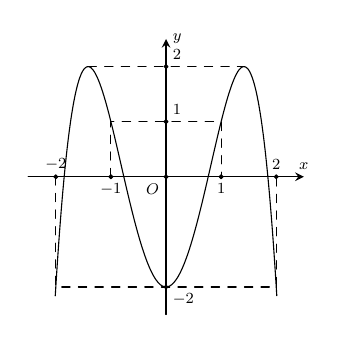
\begin{tikzpicture}[line join=round, line cap = round, >=stealth, scale=.7,font=\footnotesize,transform shape]
            \pgfmathsetmacro\a{sqrt(2)}
            \draw[->] (-2.5,0) -- (2.5,0)node[above]{$x$};
            \draw[->] (0,-2.5) -- (0,2.5)node[right]{$y$};
            %\draw[-] (-2.2,-1) -- (.75,-1) node[right]{$y=m$};
            \draw[fill=black]
            (0,0) circle(1pt) node[below left]{$O$}
            (0,2) circle(1pt) node[above right]{$2$}
            (0,1) circle(1pt) node[above right]{$1$}
            (0,-2) circle(1pt) node[below right]{$-2$}
            (2,0) circle(1pt) node[above]{$2$}
            (-2,0) circle(1pt) node[above]{$-2$}
            (-1,0) circle(1pt) node[below]{$-1$}
            (1,0) circle(1pt) node[below]{$1$}
            ;
            \draw[dashed]
            (-\a,2)--(\a,2)
            (-2,0)--(-2,-2)--(2,-2)--(2,0)
            (-1,0)--(-1,1)--(1,1)--(1,0)
            ;
            \draw[smooth,samples=100,domain=-2.01:2.01] plot(\x,{-(\x)^4+4*(\x)^2-2});
        \end{tikzpicture}
    }
    \loigiai{
        \immini{	Phương trình $f(x)=m$ có đúng $3$ nghiệm phân biệt thuộc đoạn $[-2;1]$ khi và chỉ khi đường thẳng $y=m$ cắt phần đồ thị ứng với $x\in [-2;1]$ của đồ thị hàm số $y=f(x)$ tại đúng $3$ điểm phân biệt.\\
            Nhìn vào đồ thị ta thấy điều này xảy ra khi và chỉ khi $-2<m\le 1$.\\
            Vậy phương trình đã cho có đúng $3$ nghiệm phân biệt thuộc đoạn $[-2;1]$ khi và chỉ khi $-2<m\le 1$.
        }{
            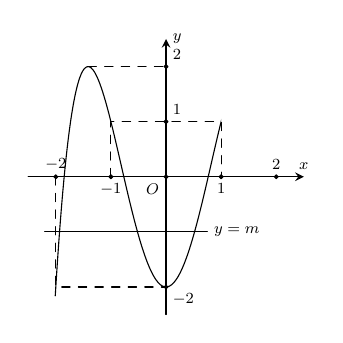
\begin{tikzpicture}[line join=round, line cap = round, >=stealth, scale=.7,font=\footnotesize,transform shape]
                \pgfmathsetmacro\a{sqrt(2)}
                \draw[->] (-2.5,0) -- (2.5,0)node[above]{$x$};
                \draw[->] (0,-2.5) -- (0,2.5)node[right]{$y$};
                \draw[-] (-2.2,-1) -- (.75,-1) node[right]{$y=m$};
                \draw[fill=black]
                (0,0) circle(1pt) node[below left]{$O$}
                (0,2) circle(1pt) node[above right]{$2$}
                (0,1) circle(1pt) node[above right]{$1$}
                (0,-2) circle(1pt) node[below right]{$-2$}
                (2,0) circle(1pt) node[above]{$2$}
                (-2,0) circle(1pt) node[above]{$-2$}
                (-1,0) circle(1pt) node[below]{$-1$}
                (1,0) circle(1pt) node[below]{$1$}
                ;
                \draw[dashed]
                (-\a,2)--(0,2)
                (-2,0)--(-2,-2)--(0,-2)
                (-1,0)--(-1,1)--(1,1)--(1,0)
                ;
                \clip (-2.5,-2.5) rectangle (1,2);
                \draw[smooth,samples=100,domain=-2.01:2.01] plot(\x,{-(\x)^4+4*(\x)^2-2});
            \end{tikzpicture}
        }
    }
\end{ex}
\begin{ex}%[2D1B5-3]
    \immini{
        Cho hàm số $y=f(x)$ có bảng biến thiên như hình vẽ. Phương trình $f(x)=m$ có ba nghiệm phân biệt khi
        \choice
        {\True $-2<m<4$}
        {$-2\leq m\leq 4$}
        {$m\in\mathbb R$}
        {$m\in\varnothing$}
    }{
        \hspace*{1cm}
        
\begin{tikzpicture}[>=stealth,scale=1]
            \tkzTabInit[nocadre=false,lgt=1.5,espcl=2]
            {$x$/1,$f'(x)$/1,$f(x)$/2}
            {$-\infty$,$-1$,$3$,$+\infty$}
            \tkzTabLine{,+,z,-,z,+,}
            \tkzTabVar{-/$-\infty$,+/$4$,-/$-2$,+/$+\infty$}
        \end{tikzpicture}
    }
    \loigiai{
        Số nghiệm của phương trình $f(x)=m$ là số giao điểm của đồ thị $y=f(x)$ và $y=m$. Do vậy, để phương trình $f(x)=m$ thì $-2<m<4$.
    }
\end{ex}
\begin{ex}%[2D1B5-3]
    \immini{Cho hàm số bậc ba $f(x)$ có đồ thị như hình vẽ. Số giá trị nguyên của tham số $m$ để phương trình $f(x)+1=m$ có ba nghiệm phân biệt là
        \choice
        {\True $3$}
        {$5$}
        {$2$}
        {$4$}}{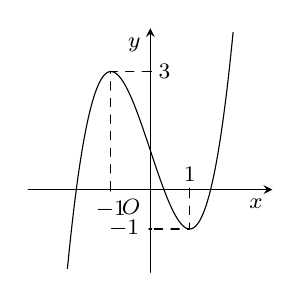
\begin{tikzpicture}[scale=0.5, font=\footnotesize, line join=round, line cap=round, >=stealth]
            \draw[->] (-3.1,0)--(3.1,0) node[below left] {$x$};
            \draw[->] (0,-2.1)--(0,4.1) node[below left] {$y$};
            \draw (0,0) node [below left] {$O$};
            \foreach \x in {-1}
            \draw[thin] (\x,1pt)--(\x,-1pt) node [below] {$\x$};
            \foreach \x in {1}
            \draw[thin] (\x,1pt)--(\x,-1pt) node [above] {$\x$};
            \foreach \y in {-1}
            \draw[thin] (1pt,\y)--(-1pt,\y) node [left] {$\y$};
            \foreach \y in {3}
            \draw[thin] (1pt,\y)--(-1pt,\y) node [right] {$\y$};
            \draw[dashed,thin](-1,0)--(-1,3)--(0,3);
            \draw[dashed,thin](1,0)--(1,-1)--(0,-1);
            \begin{scope}
                \clip (-3,-2) rectangle (3,4);
                \draw[samples=200,domain=-3:3,smooth,variable=\x] plot (\x,{1*((\x)^3)+0*((\x)^2)+-3*(\x)+1});
            \end{scope}
            % \begin{scope}[on background layer]\path[white]node{MDD-108};\end{scope}
    \end{tikzpicture}}
    \loigiai{
        Xét phương trình $f(x)+1=m \Leftrightarrow f(x) = m-1\quad (1)$.\\
        Số nghiệm của phương trình $(1)$ bằng số giao điểm của đồ thị hàm số $y=f(x)$ và đường thẳng $y=m-1$.\\
        Vậy để $(1)$ có ba nghiệm phân biệt thì $-1<m-1<3 \Leftrightarrow 0 < m < 4$.\\
        Do $m\in\mathbb{Z}$ nên $m\in\{1;2;3\}$.
    }
\end{ex}
\begin{ex}%[2D1B5-3]
    \immini
    {
        Cho hàm số $y=-2x^3+3x^2-1$ có đồ thị $(C)$ như hình vẽ. Dùng đồ thị $(C)$ suy ra tất cả giá trị tham số $m$ để phương trình $2x^3-3x^2+2m=0$ (1) có $3$ nghiệm phân biệt là
        \choice
        {\True $0<m<\dfrac{1}{2}$}
        {$-1<m<0$}
        {$0\le m\le 1$}
        {$-1\le m\le 0$}
    }
    {
        \begin{tikzpicture}[scale=.8,font=\footnotesize, line join=round, line cap=round, >=stealth]
            %%Nhập giới hạn đồ thị và hàm số cần vẽ
            \def \xmin{-2}
            \def \xmax{2.5}
            \def \ymin{-2.5}
            \def \ymax{2.5}
            \def \hamso{-2*(\x)^3+3*(\x)^2-1}
            %\def \tiemcanxien{\x+1}
            %%Tự động
            \draw[->] (\xmin,0)--(\xmax,0) node[below] {$x$};
            \draw[->] (0,\ymin)--(0,\ymax) node[left] {$y$};
            \draw (0,0) node [below right] {$O$};
            \draw (0,-1)node[below left]{$-1$};
            \draw (1,0)node[above]{$1$};
            \begin{scope}
                \clip (\xmin+0.01,\ymin+0.01) rectangle (\xmax-0.01,\ymax-0.01);
                \draw[samples=350,domain=\xmin+0.01:\xmax-0.01,smooth,variable=\x] plot (\x,{\hamso});
            \end{scope}
            % \begin{scope}[on background layer]\path[white]node{MDD-108};\end{scope}
        \end{tikzpicture}
    }
    \loigiai{
        \immini
        {
            Phương trình tương đương với $-2x^3+3x^2-1=2m-1$.\\
            Dựa vào đồ thị suy ra $-1<2m-1<0\Leftrightarrow 0<m<\dfrac{1}{2}$.
        }
        {
            \begin{tikzpicture}[scale=.8,font=\footnotesize, line join=round, line cap=round, >=stealth]
                %%Nhập giới hạn đồ thị và hàm số cần vẽ
                \def \xmin{-2}
                \def \xmax{2.5}
                \def \ymin{-2.5}
                \def \ymax{2.5}
                \def \hamso{-2*(\x)^3+3*(\x)^2-1}
                %\def \tiemcanxien{\x+1}
                %%Tự động
                \draw[->] (\xmin,0)--(\xmax,0) node[below] {$x$};
                \draw[->] (0,\ymin)--(0,\ymax) node[left] {$y$};
                \draw (0,0) node [below right] {$O$};
                \draw (0,-1)node[below left]{$-1$};
                \draw (1,0)node[above]{$1$};
                \begin{scope}
                    \clip (\xmin+0.01,\ymin+0.01) rectangle (\xmax-0.01,\ymax-0.01);
                    \draw[samples=350,domain=\xmin+0.01:\xmax-0.01,smooth,variable=\x] plot (\x,{\hamso});
                \end{scope}
                % \begin{scope}[on background layer]\path[white]node{MDD-108};\end{scope}
            \end{tikzpicture}
        }
    }
\end{ex}
\begin{ex}%[2D1B5-3]
    \immini{Cho hàm số $y=f(x)$ có đồ thị như hình vẽ bên.
        Phương trình $2f(x)+7 =0$ có bao nhiêu nghiệm?
        \choice
        {Vô nghiệm}
        {\True $4$}
        {$3$}
        {$2$}
    }
    {
        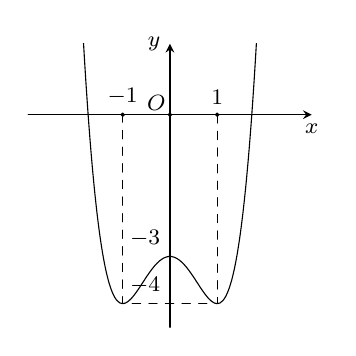
\begin{tikzpicture}[scale=0.6, font=\footnotesize, line join=round, line cap=round, >=stealth]
            \draw[->] (-3,0)--(3,0) node[below]{$x$} ;
            \draw[->] (0,-4.5)--(0,1.5) node[left]{$y$};
            \draw[fill=black] (0,0) circle(1pt) node[above left=-2pt] {$O$} ;
            \draw (1,0) circle(1pt) node[above]{$1$} (-1,0) circle(1pt) node[above]{$-1$} (0,-4) node[above left]{$-4$} (0,-3) node[above left]{$-3$};
            \draw[dashed] (1,0)--(1,-4)--(-1,-4)--(-1,0);
            \clip (-3,-4.5) rectangle (3,1.5) ;
            \draw[smooth, samples=100, domain=-3:3] plot(\x,{(\x)*(\x)*(\x)*(\x) - 2*(\x)*(\x)-3}) ;
        \end{tikzpicture}
    }
    \loigiai{
        Ta có $2f(x)+7=0 \Leftrightarrow f(x) = - \dfrac{7}{2}$. \\
        Số nghiệm của phương trình là số giao điểm của đồ thị hàm số $y=f(x)$ và đường thẳng $y=- \dfrac{7}{2}$. \\
        Do đó phương trình đã cho có $4$ nghiệm phân biệt.
    }
\end{ex}
\begin{ex}%[2D1B5-3]
    \immini{
        Cho hàm số $ y=f(x) $ có đồ thị như hình vẽ bên. Tìm tất cả các giá trị thực của tham số $ m $ để phương trình $ f(x)-m+2020=0 $ có $ 2 $ nghiệm phân biệt.
        \choice
        {$\hoac{&m>-3 \\ &m=-4 \\}$}
        {$m>2015$}
        {$m>-3$}
        {\True $\hoac{&m>2017 \\ &m=2016 \\}$}
    }{
        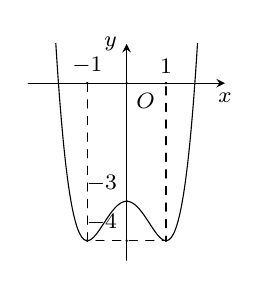
\begin{tikzpicture}[scale=.5, line cap=round,line join=round,>=stealth,x=1.0cm,y=1.0cm]
            \tkzInit[xmin=-2.5,xmax=2.5,ymax=1, ymin=-4.5]
            \draw [->](-2.5,0)--(2.5,0)node[below]{\footnotesize $x$};
            \draw [->](0,-4.5)--(0,1)node[left]{\footnotesize $y$};
            \draw[fill=black](0pt,0pt) circle (.5pt) node[below right] {\footnotesize $O$};
            \clip(-2.5,-4.5) rectangle (2.5,1);
            \draw[smooth,samples=100,domain=-2.5:2.5] plot(\x,{(\x)^4-2*(\x)^2-3});
            \foreach \x in{-1,1}\draw[fill=black](\x,0) circle (.5pt) node[above]{\footnotesize $\x$};
            \foreach \y in{-4,-3}\draw[fill=black](0,\y) circle (.5pt) node[above left]{\footnotesize $\y$};
            \draw [fill=black] (-1,-4) circle (.5pt);
            \draw [fill=black] (1,-4) circle (.5pt);
            \draw[dashed] (-1,0) |- (-1,-4)|-(1,-4) |- (1,0);
        \end{tikzpicture}
    }
    \loigiai{
        \begin{center}
            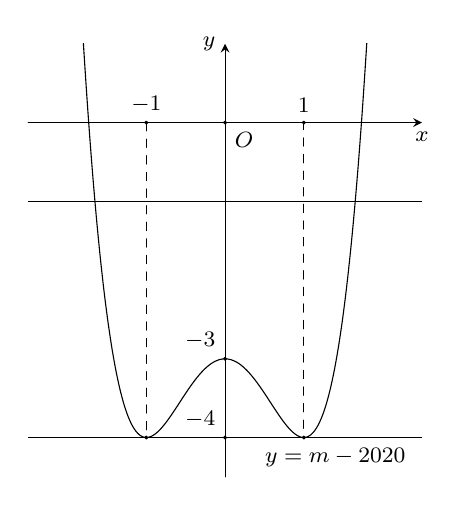
\begin{tikzpicture}[scale=1, line cap=round,line join=round,>=stealth,x=1.0cm,y=1.0cm]
                \tkzInit[xmin=-2.5,xmax=2.5,ymax=1, ymin=-4.5]
                \draw [->](-2.5,0)--(2.5,0)node[below]{\footnotesize $x$};
                \draw [->](0,-4.5)--(0,1)node[left]{\footnotesize $y$};
                \draw[fill=black](0pt,0pt)circle (.5pt) node[below right] {\footnotesize $O$};
                \clip(-2.5,-4.5) rectangle (2.5,1);
                \draw[smooth,samples=100,domain=-2.5:2.5] plot(\x,{(\x)^4-2*(\x)^2-3});
                \foreach \x in{-1,1}\draw[fill=black](\x,0) circle (.5pt) node[above]{\footnotesize $\x$};
                \foreach \y in{-4,-3}\draw[fill=black](0,\y) circle (.5pt) node[above left]{\footnotesize $\y$};
                \draw[dashed] (-1,0) |- (-1,-4)|-(1,-4) |- (1,0);
                \draw (-2.5,-4)--(2.5,-4);
                \draw (-2.5,-1)--(2.5,-1);
                \draw(1.4,-4.5) node[above]{\footnotesize $y=m-2020$};
                \draw [fill=black] (-1,-4) circle (.5pt);
                \draw [fill=black] (1,-4) circle (.5pt);
            \end{tikzpicture}
        \end{center}
        Ta có $f(x)-m+2020=0\Leftrightarrow f(x) =m-2020. \quad(*)$\\
        Số nghiệm của phương trình $(*)$ bằng số giao điểm của đồ thị hàm số $ y=f(x) $ và đường thẳng $ y=m-2020$.\\ Dựa vào đồ thị ta thấy đường thẳng $ y=m-2020$ cắt đồ thị tại $2$ điểm phân biệt khi và chỉ khi $$\hoac{&m-2020>-3\\ &m-2020=-4 \\} \Leftrightarrow \hoac{&m>2017 \\ &m=2016.}$$
        Vậy $\hoac{&m>2017 \\ &m=2016 \\}$ thỏa mãn yêu cầu bài toán.
    }
\end{ex}
\begin{ex}%[2D1B5-3]
    Tìm tất cả giá trị thực của tham số $m$ để phương trình $x^4-2x^2-m+3=0$ có hai nghiệm phân biệt.
    \choice
    {$m>3$}
    {$m\ge 3$}
    {\True $m>3$ hoặc $m=2$}
    {$m=2$ hoặc $m=3$}
    \loigiai{$x^4-2x^2-m+3=0\Leftrightarrow m=x^4-2x^2+3$.\\
        Xét $f(x)=x^4-2x^2+3$, $\mathscr{D}=\mathbb{R}$.\\
        $f'(x)=4x^3-4x$, $f'(x)=0\Leftrightarrow \hoac{&x=0\\&x=1\\&x=-1.}$\\
        Bảng biến thiên
        \begin{center}
            
\begin{tikzpicture}[>=stealth]
                \tkzTabInit[nocadre=false,lgt=1.2,espcl=2.2,deltacl=0.5]{$x$/.7 ,$f'(x)$/.7,$f(x)$/2}
                {$-\infty$ , $-1$ , $0$ , $1$ , $+\infty$}
                \tkzTabLine{ , - , $0$ , + , $0$ , - , $0$ , + , }
                \tkzTabVar{+/$+\infty$ , -/$2$, +/$3$ , -/$2$ , +/$+\infty$}
            \end{tikzpicture}
        \end{center}
        YCBT $\Leftrightarrow \hoac{&m=2\\&m>3.}$
    }
\end{ex}
\begin{ex}%[2D1B5-3]
    Cho đồ thị hàm số $y=f(x)$ như hình bên dưới. Tìm tất cả các giá trị của tham số $m$ để phương trình $f(x)+1=m$ có đúng $3$ nghiệm phân biệt.
    \begin{center}
        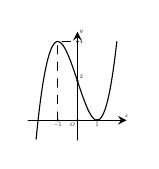
\begin{tikzpicture}[line join=round, line cap = round, >=stealth, scale=.25,font=\footnotesize,transform shape]
            \draw[->] (-2.5,0) -- (2.5,0)node[above]{$x$};
            \draw[->] (0,-1) -- (0,4.5)node[right]{$y$};
            %\draw[-] (-2.5,1) -- (2,1) node[right]{$y=m-1$};
            \draw[fill=black]
            (0,0) circle(1pt) node[below left]{$O$}
            (0,2) circle(1pt) node[above right]{$2$}
            (0,4) circle(1pt) node[right]{$4$}
            (-1,0) circle(1pt) node[below]{$-1$}
            (1,0) circle(1pt) node[below]{$1$}
            ;
            \draw[dashed]
            (-1,0)--(-1,4)--(0,4)
            ;
            \draw[smooth,samples=100,domain=-2.1:2] plot(\x,{(\x)^3-3*(\x)+2});
        \end{tikzpicture}
    \end{center}
    \choice
    {$0<m<5$}
    {\True $1<m<5$}
    {$-1<m<4$}
    {$0<m<4$}
    \loigiai{
        Ta có $f(x)+1=m \Leftrightarrow f(x)=m-1$. \quad $(*)$\\
        Phương trình $(*)$ có đúng $3$ nghiệm phân biệt khi và chỉ khi đường thẳng $y=m-1$ cắt đồ thị hàm số $y=f(x)$ tại đúng $3$ điểm phân biệt.
        \begin{center}
            \begin{tikzpicture}[line join=round, line cap = round, >=stealth, scale=1.2,font=\footnotesize,transform shape]
                \draw[->] (-2.5,0) -- (2.5,0)node[above]{$x$};
                \draw[->] (0,-1) -- (0,4.5)node[right]{$y$};
                \draw[-] (-2.5,1) -- (2,1) node[right]{$y=m-1$};
                \draw[fill=black]
                (0,0) circle(1pt) node[below left]{$O$}
                (0,2) circle(1pt) node[above right]{$2$}
                (0,4) circle(1pt) node[right]{$4$}
                (-1,0) circle(1pt) node[below]{$-1$}
                (1,0) circle(1pt) node[below]{$1$}
                ;
                \draw[dashed]
                (-1,0)--(-1,4)--(0,4)
                ;
                \draw[smooth,samples=100,domain=-2.1:2] plot(\x,{(\x)^3-3*(\x)+2});
            \end{tikzpicture}
        \end{center}
        Nhìn vào đồ thị ta thấy điều này xảy ra khi và chỉ khi $0<m-1<4 \Leftrightarrow 1<m<5$.\\
        Vậy phương trình đã cho có đúng $3$ nghiệm phân biệt khi và chỉ khi $1<m<5$.
    }
\end{ex}
\begin{ex}%[2D1B5-4]
    Biết đường thẳng $y=3x+1$ cắt đồ thị hàm số $y=\dfrac{2x^2-2x+3}{x-1}$ tại hai điểm phân biệt $A,B$ . Tính độ dài đoạn thẳng $AB$?
    \choice
    {$AB=4\sqrt{15}$}
    {\True $AB=4\sqrt{10}$}
    {$AB=4\sqrt{6}$}
    {$AB=4\sqrt{2}$}
    \loigiai{
        Phương trình hoành độ giao điểm:
        \allowdisplaybreaks
        \begin{eqnarray*}
            & &\dfrac{2x^2-2x+3}{x-1}=3x+1\\
            &\Leftrightarrow &\heva{&2x^2-2x+3=(3 x+1)(x-1)\\&x \neq 1}\\
            &\Leftrightarrow &\heva{&x^2=4\\&x \neq 1}\\
            &\Leftrightarrow &\hoac{&x=2\\&x=-2.}
        \end{eqnarray*}
        Suy ra $A(-2;-5)$, $B(2;7)$ và $AB=4\sqrt{10}$.}
\end{ex}
\begin{ex}%[2D1B5-4]
    Cho hàm số $y=2x^4-6x^2$ có đồ thị là $(C)$. Số giao điểm của đồ thị $(C)$ với đường thẳng $y=4$ là
    \choice
    {$4$}
    {\True $2$}
    {$0$}
    {$1$}
    \loigiai{
        Phương trình hoành độ giao điểm của $(C)$ và đường thẳng $y=4$ là\\ $$2x^4-6x^2=4\Leftrightarrow 2x^4-6x^2-4=0\Leftrightarrow \hoac{&x^2=\dfrac{3-\sqrt{17}}{2}\text{(vn)}\\&x^2=\dfrac{3+\sqrt{17}}{2}}\Leftrightarrow x=\pm\sqrt{\dfrac{3+\sqrt{17}}{2}}.$$\\
        Vậy số giao điểm của đồ thị $(C)$ với đường thẳng $y=4$ là $2$.
    }
\end{ex}
\begin{ex}%[2D1B5-4]
    Hàm số $y=f\left( x\right) =x^3+ax^2+bx+c$ đạt cực tiểu tại điểm $x=1$, $f\left( 1\right) =-3$ và đồ thị hàm số cắt trục tung tại điểm có tung độ bằng $2$. Tính $T=a+b+c$.
    \choice
    {$T=-2$}
    {\True $T=-4$}
    {$T=9$}
    {$T=1$}
    \loigiai{
        $f'\left( x\right) =3x^2+2ax+b$.\\
        Hàm số đạt cực tiểu tại điểm $x=1\Rightarrow f'\left( 1\right) =0\Rightarrow 2a+b=-3$.\\
        $f\left( 1\right) =-3\Rightarrow 1+a+b+c=-3\Rightarrow a+b+c=-4$.\\
        Đồ thị hàm số cắt trục tung tại điểm có tung độ bằng $2$ nên
        $f\left( 0\right) =2\Rightarrow c=2$.\\
        Ta có $\heva{&2a+b=-3\\&a+b+c=-4\\&c=2}\Rightarrow\heva{&a=3\\&b=-9\\&c=2.}$ \\
        Khi đó $f\left( x\right) =x^3+3x^2-9x+2$; $f'(x)=3x^2+6x-9$.\\
        Ta có $f'(1)=0$ $\Rightarrow x=1$ là điểm cực tiểu.\\
        Vậy $T=a+b+c=-4$.}
\end{ex}
\begin{ex}%[2D1B5-4]
    Tìm số giao điểm của đồ thị hàm số $y=x^4+2x^2-m^2-1$ với trục hoành ($m$ là tham số thực).
    \choice
    {$1$}
    {\True $2$}
    {$3$}
    {$4$}
    \loigiai{Phương trình hoành độ giao điểm $x^4+2x^2-m^2-1=0\Leftrightarrow x^4+2x^2-1=m^2$.\\
        Xét $f(x)=x^4+2x^2-1$, $\mathscr{D}=\mathbb{R}$.\\
        $f^\prime(x)=4x^3+4x$, $f^\prime(x)=0\Leftrightarrow x=0$.\\
        Bảng biến thiên
        \begin{center}
            
\begin{tikzpicture}[>=stealth]
                \tkzTabInit[nocadre=false,lgt=1,espcl=2,deltacl=0.5]{$x$/.7 ,$y'$/.7,$y$/2}
                {$-\infty$ , $0$ , $+\infty$}
                \tkzTabLine{ , - , $0$ , + , }
                \tkzTabVar{+/$+\infty$ , -/$-1$ , +/$+\infty$}
            \end{tikzpicture}
        \end{center}
        Do $m^2\ge 0>-1$ nên đường thẳng $y=m^2$ luôn cắt đồ thị hàm số $y=x^4+2x^2-1$ tại hai điểm phân biệt.
    }
\end{ex}
\begin{ex}%[2D1B5-4]
    Biết đường thẳng $y=x-2$ cắt đồ thị hàm số $y=\dfrac{2x+1}{x-1}$ tại hai điểm phân biệt $A$, $B$ có hoành độ lần lượt ${x_A}$, ${x_B}$. Khi đó ${x_A}+{x_B}$ là
    \choice
    {\True ${{x}_A}+{{x}_B}=5$}
    {${{x}_A}+{{x}_B}=2$}
    {${{x}_A}+{{x}_B}=3$}
    {${{x}_A}+{{x}_B}=1$}
    \loigiai{
        Xét phương trình hoành độ giao điểm
        $$\dfrac{2x+1}{x-1}=x-2\Leftrightarrow\heva{&x\ne 1\\
            & 2x+1=\left(x-1\right)\left(x-2\right)\\
        }
        \Leftrightarrow\heva{& x\ne 1\\
            & x^2-5x+1=0\quad\left(*\right)\\
        }$$
        Ta thấy $\left( * \right)$ có 2 nghiệm thực phân biệt ${x_A}$, ${x_B}$ khác $1$ và ${x_A}+{x_B}=5$.}
\end{ex}
\Closesolutionfile{ans}